\lab{Algorithms}{Givens rotations and Least squares}{Givens rotations and Least squares}
\objective{Use orthogonal transformations to perform QR decomposition.}
\label{lab:givens}

In a previous lab, we discussed how to form the QR decomposition of a matrix using a series of householder reflectors.
The general approach was to apply a series of orthogonal transformations to a given matrix to transform it into upper triangular form.
This same approach can be applied using rotations instead of reflections.

The matrix $\begin{pmatrix}\ cos \theta & - \sin \theta \\ \sin \theta & \cos \theta \end{pmatrix}$ rotates a vector counterclockwise by $\theta$.
Given a vector $x = \begin{pmatrix} a \\ b \end{pmatrix}$, we can rotate $x$ into the span of $e_1$ by choosing the correct $\theta$.
This zeros out the entry containing $b$.
We could do this by finding the angle between $\begin{pmatrix} a \\ b \end{pmatrix}$ and the axis containing $b$ then rotating the vector by the negative of that angle.
In order to avoid computations involving $\sin$ and $\arcsin$ at each iteration we can just solve for $\sin \theta $ and $\cos \theta$ using the pythagorean theorem instead of explicitly computing $\theta$.
Such an approach gives us the result that $\cos \theta = \frac{a}{\sqrt{a^2 + b^2}}$ and $\sin \theta = \frac{- b}{\sqrt{a^2 + b^2}}$.
The transformed image of $\begin{pmatrix} a \\ b \end{pmatrix}$ is then $\begin{pmatrix} \sqrt{a^2 + b^2} \\ 0 \end{pmatrix}$.

The application of such a rotation to any two rows of a matrix $A$ is an orthonormal transform.
Such a transformation can be represented in matrix form, where $c = \cos \theta$ and $s = \sin \theta$, like this:
\begin{equation*}
\begin{pmatrix}
I & 0 & 0 & 0 & 0 \\
0 & c & 0 & -s & 0 \\
0 & 0 & I & 0 & 0 \\
0 & s & 0 & c & 0 \\
0 & 0 & 0 & 0 & I
\end{pmatrix}
\end{equation*}
In actual computation, we \emph{do not} actually form such a large matrix at each step.
Instead we apply the transformation to the two rows we want to change and then leave the rest of the matrix unchanged.
Proceeding in this manner we can zero out each entry of any matrix below its main diagonal, resulting in a QR factorization.
For an example, consider some matrix $A$.
Let $G \left( i, j, k \right)$ denote the Givens rotation that will zero out $A \left[ j, k \right]$ by rotation with row $i$ of $A$.
We can zero out the entries below the main diagonal of A as follows:

\[
\begin{array}{ccccccc}
\begin{pmatrix}
*&*&*\\
*&*&*\\
*&*&*
\end{pmatrix}
&
\underrightarrow{G(1,2,0)}
&\begin{pmatrix}
*&*&*\\
*&*&*\\
0&*&*
\end{pmatrix}
&
\underrightarrow{G(0,1,0)}
&\begin{pmatrix}
*&*&*\\
0&*&*\\
0&*&*
\end{pmatrix}
&
\underrightarrow{G(1,2,1)}
&\begin{pmatrix}
*&*&*\\
0&*&*\\
0&0&*
\end{pmatrix}
\end{array}
\]

Here is an outline for the algorithm.
Let $A$ be the array passed to the function.

\begin{comment}

\begin{algorithm}
\begin{algorithmic}[1]
\Procedure{Givens Triangularization}{$A$}
\State $R \gets \text{copy}(A)$
\State $Q \gets I_A$
\State $G \gets \text(empty)(2,2)$
\For{each column}
    \For{each row below the main diagonal}
        \If{leading element is not zero}
            \State Compute $c$ and $s$ using the entry in the current row and column and the entry immediately above it
            \State Use $c$ and $s$ to construct the matrix $G$
            \State Get a slice of $R$ of the current row and the row above it that includes the columns from the current column onward.
                Multiply it in place by $G$ to zero out the leading nonzero entry of the current row.
            \State Get a slice of $Q$ of the current row and the row above it and apply $G$ to it as well.
                (Strictly speaking, you do not need to operate over these entire rows, but the slicing needed to avoid the extra computation is a little more involved, so we will not include that here.)
        \EndIf
    \EndFor
\EndFor
\State \pseudoli{return} $Q^T, R$
\EndProcedure
\end{algorithmic}
\end{algorithm}

\end{comment}

\begin{itemize}[$\bullet$]

\item Make $R$ a copy of $A$ and $Q$ an identity array of the appropriate size.

\item Make an empty $2 \times 2$ array $G$ that will be used to apply the Givens rotations.

\item For each column:

  \begin{itemize}[$\bullet$]

  \item For each row below the main diagonal (starting at the bottom of the column):

    \begin{itemize}[$\bullet$]

    \item If the leading entry of this row is not zero (i.e. if its absolute value is within a given tolerance):

      \begin{itemize}[$\bullet$]

      \item Compute $c$ and $s$ using the entry in the current row and column and the entry immediately above it.

      \item Use $c$ and $s$ to construct the matrix $G$.

      \item Get a slice of $R$ of the current row and the row above it that includes the columns from the current column onward.
      Multiply it in place by $G$ to zero out the leading nonzero entry of the current row.

      \item Get a slice of $Q$ of the current row and the row above it and apply $G$ to it as well. (Strictly speaking, you do not need to operate over these entire rows, but the slicing needed to avoid the extra computation is a little more involved, so we will not include that here.)

      \end{itemize}

    \end{itemize}

  \end{itemize}

\item Return $Q^T$ and $R$.

\end{itemize}

This version of the algorithm is not the most well-optimized way to use Givens rotations, but it is good for illustrative purposes.

Because Givens rotations only operate on two specific rows at a time, they give us a variety of ways to iterate over an array we are processing.
For example, using Givens rotations you could, starting at the bottom of each column and continuing up until you reach the main diagonal, zero out each entry by applying a Givens rotation to each row and the row immediately above it.
Alternatively, within each column, you could could zero out the first entry of each row below the main diagonal by rotating it with the row corresponding to the main diagonal.
Yet another way to do it would be to start at the bottom left corner of the matrix and then zero out each entry from left to right along each diagonal.
This flexibility is what makes the use of Givens rotations ideal for some problems.
When working with sparse matrices, Givens rotations allow for the solution of linear systems through a series of orthonormal operations that operate only on small parts of the array.
The fact that Givens rotations operate only on small portions of the array also lends well to parallel solutions to systems of equations (or least squares problems).
They allow for the sort of flexibility we had when using Gaussian elimination while still maintaining the favorable stability that comes with using orthonormal transformations.

While Givens rotations do allow for greater flexibility, they also require a greater number of floating point operations than Householder reflections.
In general, the operation count for computing the QR factorization for an $m \times n$ matrix is $3 n^2 \left( m - \frac{n}{3} \right)$.
% Accuracy and Stability of Numerical Algorithms, Nicholas J. Higham
There are modified versions of the Givens QR algorithm that use ``fast Givens rotations" which decrease the number of multiplications and square roots needed for the application of each Givens rotation.
% Fast Plane Rotations With Dynamic Scaling, Anda and Park, SIAM, 1994
It allows for the use of Givens rotations while requiring roughly the same number of floating point operations used by the Householder QR algorithm.
In practice, these methods are still not quite as fast as the Householder algorithm.
In spite of the need for more floating point operations, Givens rotations are still well suited for parallelization and can be much faster than the Householder algorithm when multiple processors are used.
% Givens and Householder Reductions for Linear Least Squares on a Cluster of Workstations, Omer Egecioglu and Ashok Srinivasan

\begin{problem}
\label{prob:Givens}
Write a function called \li{givens} that uses Givens rotations to compute the $QR$ decomposition of
a matrix $A$.
By performing successive Givens rotations, triangularize $A$ to find $R$.
Apply the rotations to an identity matrix as you go, then take the transpose to invert it and find $Q$.
Return $Q$ and $R$.
\end{problem}

We will now illustrate one example of how to use Givens rotations to change only specific parts of the array.

\begin{problem}
\label{prob:givens_hessenberg}
Write a modified version of your solution to Problem \ref{prob:Givens}, call it \li{givens2} that computes the 
QR decomposition of an upper Hessenberg matrix.
Instead of starting at the bottom of each column and working up, just run down the first subdiagonal from left to right.
When operating on $Q$, you do not need to operate on the full length of each row.
It is sufficient to perform the matrix multiplication on the portion of the array \li{Q[j:j+2,:j+2]} where \li{j} is the current column.

Note: You can zero out the portion below the first subdiagonal of a matrix like this:
\begin{lstlisting}
import numpy as np
import scipy.linalg as la
from numpy.random import rand
A = rand(500, 500)
A[1:] = la.triu(A[1:])
\end{lstlisting}

Notice how $Q$ in the QR decomposition of an upper Hessenberg matrix is also upper Hessenberg.
What is the computational order of  complexity for this problem?
Approximately for what $m$ is your implementation as fast as the general QR decomposition built in to \li{scipy.linalg} for computing the QR decomposition of an upper Hessenberg matrix?
\end{problem}

\begin{problem}
\label{prob:givens_hessenberg_modified}
You may have noticed that matrix multiplication by $Q$ is generally a $\mathcal{O} \left( n^3 \right)$ algorithm, while the application of these individual Givens rotations is a $\mathcal{O} \left( n^2 \right)$ algorithm.
Write a modified version of your solution to Problem \ref{prob:givens_hessenberg} called \li{givens2_mod} which returns 
an $(n-1) \times 2 \times 2$ array containing the computed values for $G$ at each step in the algorithm in the order in which they are applied to the upper Hessenberg array $H$.

Write two more functions \li{apply_Q} and \li{apply_QT} which, using the matrix of Givens rotations, perform left multiplication 
by $Q$ and $Q^{-1}$, respectively, on some other input array $B$.
Left multiplication by $Q^{-1}$ can be done by applying each of the Givens rotations to $B$ the same way you did to $H$ to compute its QR factorization.
Left multiplication by $Q$ can be done by applying the transpose of the Givens rotations to their corresponding portions of $B$, but in the reverse order.
Notice that you will have to apply each Givens rotation across the full width of the rows it operates on since you do not know anything about the content of $B$.

For around what size of matrices is direct multiplication by $Q$ slower than this method of multiplying by $Q$?
For timing purposes, make a random upper Hessenberg matrix, compute its QR decomposition using the function you just wrote and your solution to Problem \ref{prob:givens_hessenberg}, then time how long it takes to left multiply a random square array by $Q$ using the function you just wrote and the \li{dot} method of NumPy arrays.

Note: the functions you just wrote can be used to perform right multiplication as well since $B Q = \left(Q^T B^T \right)^T$ and $B Q^T = \left( Q B^T \right)^T$.
\end{problem}

An interesting side-note is that each Givens rotation can be represented as a single floating point number, so, when operating in place, $Q$ can be stored entirely in the lower triangular portion of the array on which we are operating by storing each rotation in the entry that it zeroes out.
A similar approach would to store Householder reflectors in the columns they zero out.
In either case, we can represent the QR decomposition of an array using only the memory that was originally used to store the array itself.
This is similar to the approach  for computing the LU decomposition entirely in place.
These representations of $Q$ and $R$ can be used in various ways to perform matrix multiplication by $Q$, $Q^T$ and $R$ as needed.

\section*{Least Squares}

We are now changing the subject to talk about line fitting.

It is well known that the displacement of a spring is proportional
to the force acting upon it, that is, $F = k x$.  The proportionality
constant $k$ is called Hooke's spring constant.  Consider a laboratory
experiment where different loads are placed on a spring and the displacement
is measured and recorded in the table below:
\vspace{5mm}\\
\begin{center}
\begin{tabular}{|c|c|}
	\hline
x & F \\
(cm) & (dyne)\\
\hline
1.04  & 3.11 \\
2.03  &  6.01\\
2.95  &  9.07\\
3.92  &  11.99\\
5.06  &  15.02\\
6.00  &  17.91\\
7.07  &  21.12\\
\hline
\end{tabular}
\end{center}
\vspace{5mm}
To find the spring constant $k$, we simply need to solve the following linear system
\[
\begin{pmatrix}
1.04\\
2.03\\
2.95\\
3.92\\
5.06\\
6.00\\
7.07\\
\end{pmatrix}
\begin{pmatrix}k\end{pmatrix} =
\begin{pmatrix}
3.11 \\
6.01\\
9.07\\
11.99\\
15.02\\
17.91\\
21.12\\
\end{pmatrix}.
\]
However, there is no solution to this system because it is overdetermined.
Instead, we seek the ``best'' $k$ that fits the data.
Least squares allows us to find that ``best'' solution.
We can find the least squares solution by computing the following in Python:
\begin{lstlisting}
>>> import numpy as np
>>> from scipy import linalg as la
>>> A = np.vstack([1.04,2.03,2.95,3.92,5.06,6.00,7.07])
>>> b = np.vstack([3.11,6.01,9.07,11.99,15.02,17.91,21.12])
>>> k = np.dot(np.dot(la.inv(np.dot(A.T,A)),A.T),b)
>>> k
array([[ 2.99568294]])
\end{lstlisting}
Hence, we find the spring constant to be $k = 2.9957$.
Note that \li{scipy.linalg} provides a built-in function for solving
least-squares problems.
We plot the data against the best fit as follows:
\begin{figure}[h!]
\label{fig1}
\begin{center}
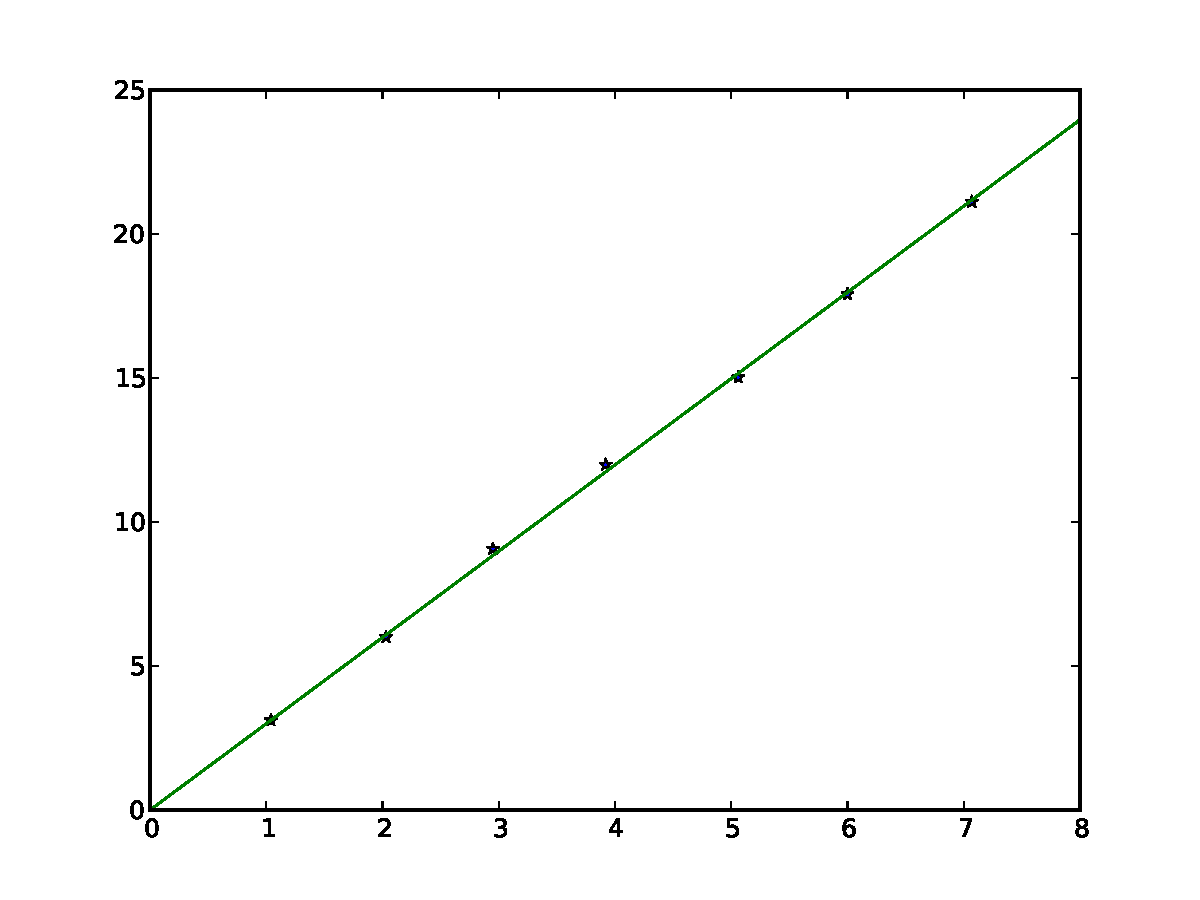
\includegraphics[width=\textwidth]{line_lstsq}
\caption{The graph of the spring data together with its linear fit}
\label{Fig:SpringFit}
\end{center}
\end{figure}

\begin{lstlisting}
>>> from matplotlib import pyplot as plt
>>> x0 = np.linspace(0,8,100)
>>> y0 = k[0]*x0
>>> plt.plot(A,b,'*',x0,y0)
>>> plt.show()
\end{lstlisting}
See Figure \ref{Fig:SpringFit} to see how well the line fits the data.


\section*{General Line Fitting}

Suppose that we wish to fit a general line, that is $y=m x+b$, to the data set
$\{(x_k,y_k)\}^n_{k=1}$.  Assume that the line does not cross through the origin,
as in the previous example.  Then we seek both a slope and a $y$-intercept.
In this case, we set up the following linear system $A x = b$, or more precisely
\[
\begin{pmatrix}
x_1 & 1\\
x_2 & 1\\
x_3 & 1\\
\vdots & \vdots\\
x_n & 1
\end{pmatrix}
\begin{pmatrix}
m\\
b
\end{pmatrix}=
\begin{pmatrix}
y_1\\
y_2\\
y_3\\
\vdots\\
y_n
\end{pmatrix}.
\]
Note that $A$ has rank $2$ as long as not all of the $x_k$ values are the same.
Hence, the least squares solution
is given by
$$
\widehat{x} = (A^HA)^{-1}A^Hb.
$$
In what sense does this solution give us the best fit line for the data? Recall that since $A$ is injective,
the matrix $A(A^HA)^{-1}A^H$ is an orthogonal projector onto the range of $A$, which means that
$A(A^HA)^{-1}A^Hb = A\widehat{x}$ is the closest vector (with respect to the 2-norm) to $b$ that lies in the
range of $A$. That is, $\widehat{x}$ minimizes the error between $Ax$ and $b$, where the error is given
by the distance between these vectors, $\|b-Ax\|_2$. Another way to say this is that $\widehat{x}$ gives the
values $m$ and $b$ for which the sum of the squares of the distances from each data point $y_k$ to the value
$y = mx_k + b$ is as small as possible.

\section*{Loading Data from .npz Files}
For Least Squares problems as well as in many other contexts, loading data is often a necessary step before
proceeding with further analysis. Here we briefly review another data format in Python and the commands used
to load the data.

A \li{.npz} file is a compressed binary file that contains an archive of NumPy data structures.
A given file may therefore contain several arrays, each array associated with a unique string that identifies it.
When you load a \li{.npz} file in Python, a dictionary-like object is returned, and you can access the data by
providing the appropriate key. Note that when you load a \li{.npz} file, you must also be sure to close it when
you are finished. This is taken care of automatically if you use the \li{with ... as} keywords.

As an example, suppose that we have a file named \li{grades.npz} that contains several arrays, each giving the
homework scores of a particular student in a particular class. Assuming that one of the arrays is associated with
the key \li{'Abe'}, we can load this array in the following way:

\begin{lstlisting}
>>> with np.load('grades.npz') as grades:
>>>     abe_grades = grades['Abe']
>>> abe_grades
array([ 10.,  10.,  10.,  10.,  10.,  10.,  10.,  10.,  10.,  10.])
\end{lstlisting}

You will need to apply this technique in the next problem.

\begin{problem}
Write a function \li{fitLine} that takes no arguments and executes the following.
Load the \texttt{linepts} array from \texttt{data.npz}.
This consists of two columns corresponding to the $x$ and $y$ values of a given data set.
Use least squares to find the slope and $y$-intercept that best fits the data.
Then plot the data points and the line on the same graph.
The function should not return anything.
\end{problem}

\section*{Fitting data to a circle}

Recall that the equation of a circle, with radius $r$ centered at $(c_1,c_2)$, is given by
\begin{equation}
\label{circle}
(x-c_1)^2 + (y-c_2)^2 = r^2.
\end{equation}
Suppose we are given a set of data points closely forming a circle $\{(x_i,y_i)\}^n_{i=1}$.
The ``best'' fit is found via least squares by expanding \eqref{circle} to get
\[
2 c_1 x + 2 c_2 y + c_3 = x^2 + y^2,
\]
where $c_3 = r^2 - c_1^2 - c_2^2$.  Then we can write the linear system $A x = b$ as
\[
\begin{pmatrix}
2 x_1 & 2 y_1 & 1\\
2 x_2 & 2 y_2 & 1\\
\vdots & \vdots & \vdots \\
2 x_n & 2 y_n & 1
\end{pmatrix}
\begin{pmatrix}
c_1\\
c_2\\
c_3
\end{pmatrix}=
\begin{pmatrix}
x_1^2 + y_1^2\\
x_2^2 + y_2^2\\
\vdots\\
x_n^2 + y_n^2
\end{pmatrix},
\]
where the matrix $A$ and the vector $b$ are obtained by the given data and the unknown
$x$ contains the information about the center and radius of the circle and is obtained
by finding the least squares solution.

\section*{Example}

In this section, we fit the following points to a circle:
\begin{align*}
&(134,76),(104,146),(34,176),(-36,146),\\
&(-66,76),(-36,5),(34,-24),(104,5),(134,76)
\end{align*}

We enter them into Python as a $9\times 2$ array:
\begin{lstlisting}
>>> P = np.array([[134,76],[104,146],[34,176],[-36,146],
                  [-66,76],[-36,5],[34,-24],[104,5],[134,76]])
\end{lstlisting}
We compute $A$ and $b$ by entering the following:
\begin{lstlisting}
>>> A = A =np.hstack((2*P, np.ones((9,1))))
>>> b = (P**2).sum(axis=1)
\end{lstlisting}
Hence, we get the least squares solution
\begin{lstlisting}
>>> x = np.dot(np.dot(la.inv(np.dot(A.T,A)),A.T),b)
\end{lstlisting}
Then we find $c_1$, $c_2$, and $r$ by:
\begin{lstlisting}
>>> from math import sqrt
>>> c1, c2, c3 = x
>>> r = sqrt(c1**2 + c2**2 + c3)
\end{lstlisting}
We plot this by executing
\begin{lstlisting}
>>> theta = np.linspace(0,2*np.pi,200)
>>> plt.plot(r*np.cos(theta)+c1,r*np.sin(theta)+c2,'-',P[:,0],P[:,1],'*')
>>> plt.show()
\end{lstlisting}


\begin{problem}
Write a function \li{fitCircle} that does the following.
Load the \texttt{circlepts} array from \texttt{data.npz}.
This consists of two columns corresponding to the $x$ and $y$ values of a given
data set.  Use least squares to find the center and radius of the circle that best
fits the data.  Then plot the data points and the circle on the same graph.
The function should return nothing.
\end{problem}

\begin{problem}
The general equation for an ellipse is:
\[
ax^2 + bx + cxy + dy + ey^2 = 1
\]

Write a function \li{fitEllipse} that uses least squares to fit data to an ellipse.
The function should take a $n\times 2$ array as input, where the first column gives the $x$-coordinates
and the second column gives the $y$-coordinates. Find the least squares solution for $a, b, c, d,$ and $e$,
and return the solution.
You can test out your function on the \texttt{ellipsepts} array from \texttt{data.npz}. You should get  $0.087$, $-0.141$,  $0.159$, $-0.316$, $0.366$ for $a, b, c, d,$ and $e$ respectively.
\end{problem}

In these Least Squares problems, we have found best fit lines and ellipses relative to the 2-norm.
It is possible to generalize the idea of best fit curves relative to other norms.
See Figure \ref{Fig:ellipse} for an illustration of this.

\begin{figure}[h]
\label{ellipsefit}
\centering
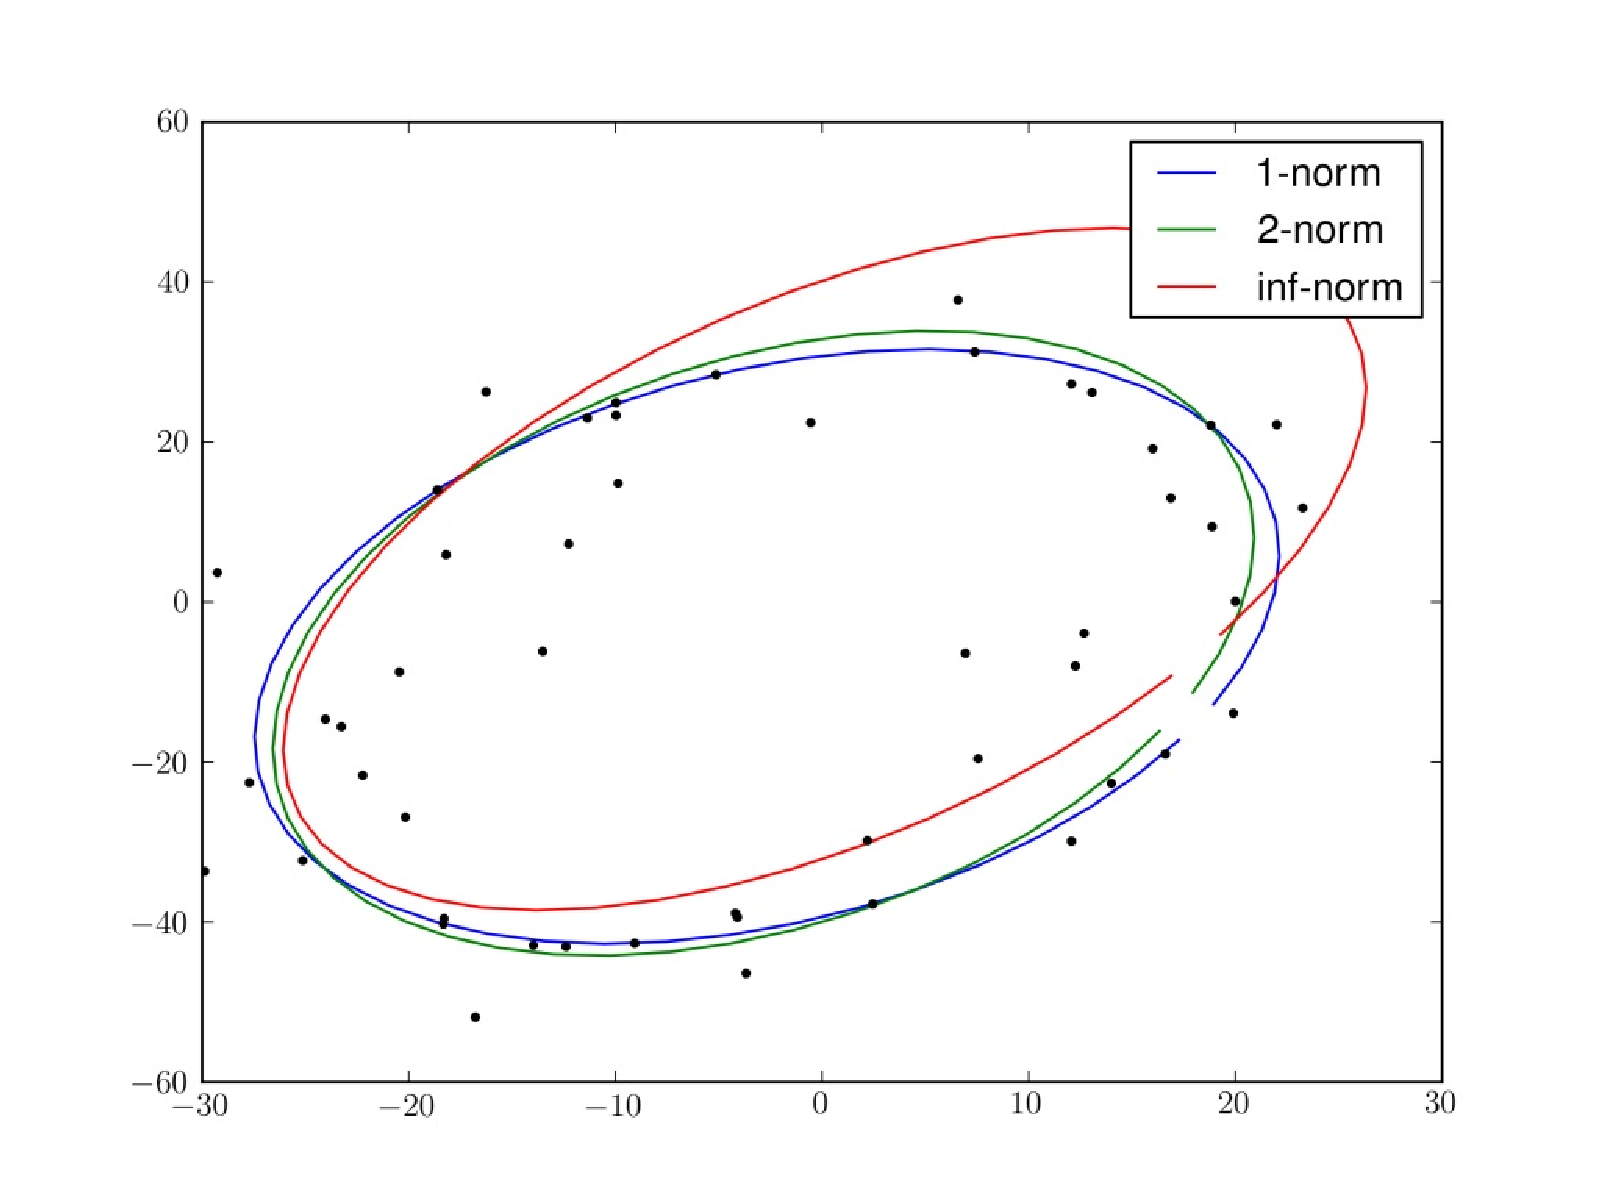
\includegraphics[width=\textwidth]{ellipsefit.pdf}
\caption{Fitting an ellipse using different norms.}
\label{Fig:ellipse}
\end{figure} 

COPIED FROM PREVIOUS LAB

\section*{Solving Least Squares Problems}
The QR decomposition can only be used to solve the linear least squares problem if $A$ is full rank. If $A$ is less than full rank, then we have to calculate the least squares solution more creatively.

%MATLAB's least squares backslash operator is based off the QR decomposition.
%SciPy uses the SVD to solve least squares problems because, although it is slower, the algorithm is more numerically stable.


For large or ill-conditioned problems, the QR decomposition provides a nice method for computing least squares solutions of over-determined matrices.
Consider the least squares problem $Ax=b$. We can approximate the solution with $\widehat x = (A^T A)^{-1}A^T b$.
Alternatively, we write the linear system as
\[ Q R x = b. \]
We then multiply both sides by $Q^T$, yielding
\[ R x = Q^T b. \]
Then $\widehat x = R^{-1} Q^T b$.

However, we can avoid calculating the inverse of $R$ (inverting a matrix is \emph{very expensive} computationally).
Since $R$ is a triangular matrix, we have a triangular system that we can solve much more efficiently.
SciPy includes a solver for triangular systems, \li{linalg.solve_triangular()}.
We approximate $x$ by solving the triangular system $Rx = Q^T b$.

\begin{problem}
Write a function \li{LeastSquares} that will accept a linear system (a matrix $A$ and a vector $b$) and solve the least squares problem.
Your function should rely on the SciPy's QR decomposition and triangular system solver.  Assume that $A$ is full rank.
You may test your function against the output of SciPy's least squares function, \li{linalg.lstsq()}.
\end{problem}


